
Define a matrix $\vec{M}$ such that,
\begin{align}
    \vec{M} &= \myvec{\vec{B-A} & \vec{C-A}}^T\\
    \vec{M} &= \myvec{-1 & -4\\4 & -1}
\end{align}
Using matrix transformation,
\begin{align}
    \vec{M} = \myvec{-1 & -4\\4 & -1}\xleftrightarrow{R_1\leftarrow -R_1 - \frac{R_2}{4}} \myvec{0 & \frac{17}{4}\\4 & -1}\\
    \implies rank(\vec{M}) = 2
\end{align}
Since the rank of matrix $\vec{M}$ is 2, the points form a triangle.
\begin{align}
    AB^2 &= \brak{\vec{A} - \vec{B}}^T\brak{\vec{A} - \vec{B}}\\
    &= 17\\
    BC^2 &= \brak{\vec{B} - \vec{C}}^T\brak{\vec{B} - \vec{C}}\\
    &= 34
    \\
    CA^2 &= \brak{\vec{C} - \vec{A}}^T\brak{\vec{C} - \vec{A}}\\
    &= 17
    \\
    \implies AB &= AC
\end{align}
Hence, the triangle is isosceles.  See Fig.     \ref{rams/1/1/6fig:plot}
\begin{figure}[htp]
    \centering
    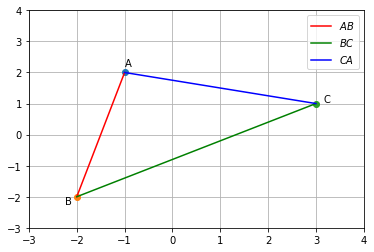
\includegraphics[width=\columnwidth]{solutions/1/1/6/Figures/Fig1.png}
    \caption{Plot of the given points}
    \label{rams/1/1/6fig:plot}
\end{figure}

